\documentclass{ttithesis}

\usepackage{amsmath}
\usepackage{graphicx}
\usepackage{scrextend}
\usepackage{setspace}
\usepackage{color}
\usepackage{tabularx}


\title{文書・文間及びカテゴリ間の関係を考慮した\\レーティング予測}
\author{12056\hspace{16ex}外山洋太}
\date{平成28年 2月}
\laboratory{知能数理研究室}



\begin{document}

\section{序論} \label{sec:Introduction}

本研究は多カテゴリにおけるレーティング予測に関する研究である。
以下に、研究背景と目的、及び、提案手法の概略、本研究の貢献を示す。
最後に論文全体の構成を示す。

\subsection{背景}

企業がマーケティングのために行う商品の評判分析において、
商品レビューに対するレーティング予測は重要な要素技術のひとつである。
何万件という大量のレビューデータを人手で処理することは難しく、
計算機による自動化が望まれる。
その中で商品を複数のカテゴリにおいてレーティング予測をする問題がある。
カテゴリとは、宿泊施設のレビューを例にすると、サービス、立地、食事等の
レーティングが付けられる各項目のことである。
この問題に関する従来手法\cite{fujitani15}は、文間の関係性を考慮しておらず、
カテゴリ間については考慮しているものの複雑な関係を考慮できていない。

近年、そのレーティング予測において、ニューラルネットワークを用いた手法
\cite{nal14,rie14,duyu15}が
提案されており、従来の手法を上回る正答率を達成している。
ニューラルネットワークをレーティング予測に用いる利点はまず
層の数を増やすことによって入力の複雑な繋がりを考慮できることである。
例えば、文毎の素性を入力とすれば文間の関係を考慮することができる。
さらに、多カテゴリにおけるレーティング予測では
カテゴリ間の関係を考慮した予測が実現できる。
しかし、レーティング予測に関する多くの研究は1つのカテゴリにおける
二値または多値分類問題を対象としている。

文や文書の意味表現の学習手法として、単語と文書の分散表現を同時に学習する
パラグラフベクトル\cite{quoc14}がある。
これはレーティング予測において優れた性能を示している。
しかし、文書全体にパラグラフベクトルを用いた場合、
レーティングの予測時に文間の関係を考慮できない。


\subsection{目的}

複数カテゴリにおけるレーティング予測について、
文書及び文間の関係とカテゴリ間の関係を同時に考慮したものの実現を目的とする。
これにより、提案手法が従来手法\cite{fujitani15}より高い正答率を
達成することを目指す。
また、実際に文書・文間の関係の考慮がレーティング予測の正答率向上に
有効であるか検証する。


\subsection{提案手法}

提案手法はパラグラフベクトルと\nn を用いたレーティング予測の手法である。
提案手法では、まずパラグラフベクトル\cite{quoc14}によって
各レビューの文書ベクトルと文ベクトルを生成する。
次に、各レビューの文ベクトルをその位置によって重み付け平均する。
これにより、文の大まかな位置関係を保持したまま
レビュー間の文ベクトルの数を固定にする。
最後に、その文書ベクトルと重み付け平均された文ベクトルを
\nn による分類器によって分類しレーティング予測を行う。


\subsection{貢献}

本研究の貢献は2つある。
1つ目は、レーティングの付けられていない
一般の商品の批評文書から多カテゴリにおけるレーティングを、
従来手法より高い正答率で予測できるようになったことである。
これによって、企業は多様な文書から自社の商品のレーティングを複数の観点で
分析できる。
2つ目は、ユーザが付与したものより客観的なレーティングを
各商品レビューに対して予測できることである。
各商品レビューのレーティングはそれぞれのユーザが付与するため、
個々のユーザの主観による影響が大きい。
しかし、機械学習によるレーティング予測では、
大量の商品レビューから学習した結果から
各レビューに対してレーティングを予測する。
そのため、ユーザの主観による影響を大きく減らすことができる。
これは、企業が個々の商品レビューを分析する際に役立つ。

%本研究は、多カテゴリにおけるレーティング予測について、
%従来手法\cite{fujitani15}より高い正答率を示す手法を提案した。
%提案手法は、レーティング不可能という意味を持った
%レーティング値の予測において従来手法より特に優れていることが分かった。
%また、レーティング予測において文書・文ベクトルを同時に用いることが
%有効であることを示した。
%これは同時に、文書ベクトルと文ベクトルがいくらか異なる特徴を捉えていることを
%示す。
%さらに、文ベクトルの位置関係の考慮がレーティング予測に重要であることを示した。

%\subsection{構成}
%
%本論文は本節を含む6節からなる。
%%\secref{sec:Introduction}は本節であり、本研究の背景、目的、
%%研究分野への貢献、論文の全体の構成について述べる。
%\secref{sec:RelatedResearch}では、本研究の従来手法\cite{fujitani15}と、
%提案手法がレーティング予測のために用いるいくつかの手法、研究について述べる。
%\secref{sec:ProposedMethod}では、提案手法の基礎となる考えと
%その具体的なアルゴリズムについて説明する。
%\secref{sec:Experiments}では、提案手法と従来手法、及び、3つの比較手法を
%用いた実験の実験設定と結果について説明する。
%\secref{sec:Discussion}では、実験結果とそれによって明らかとなった
%提案手法の性質について考察する。
%また、提案手法の問題点からその改善方法について議論する。
%\secref{sec:Conclusion}では、まとめと今後の予定について述べる。

\section{関連研究} \label{sec:RelatedResearch}

\subsection{隠れ状態を用いたホテルレビューのレーティング予測}

藤谷ら\cite{fujitani15}は複数のカテゴリにおけるレーティング予測に対して、
Multi-Instance Multi-Label learning for Relation Extraction (MIML-RE)
\cite{mihai12}モデルを用いた手法を提案している。
その手法では、レビュー内の各文毎に予測した隠れレーティングから
レビュー全体のレーティングを予測する。
図\ref{fig:FujitaniRelationsAmongRatingCategories}のように、
文毎のレーティングからレビュー全体のレーティングを予測する際の
カテゴリ間の繋がりを手動で変化させカテゴリ間の関係性を考慮している。
各文の素性にはBag Of Words (BOW)またはBag Of n-gramsを用いている。
各文毎に隠れレーティングを予測することによって
0.4832の正答率が得られることが示された。
また、カテゴリ間の繋がりによって正答率が変化することも示されている。

\begin{figure}
  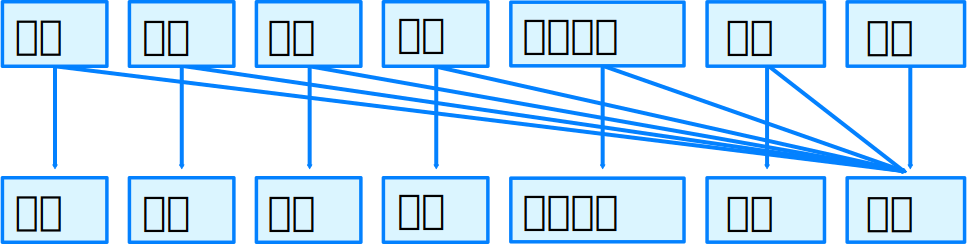
\includegraphics[0.5]
      {fig/fujitani_miml_relations_among_rating_categories.pdf}
  \caption{藤谷ら\cite{fujitani15}のモデルにおけるカテゴリ同士の繋ぎ方の例}
  \label{fig:FujitaniRelationsAmongRatingCategories}
\end{figure}

この手法では、文同士の位置関係を考慮しておらず、
カテゴリ間については考慮しているものの複雑な関係を捉えることができていない。

\subsection{パラグラフベクトル}

パラグラフベクトルは、文や文書といった大きな単位の言語表現の意味表現を
学習する手法である。
これは、Continuous BOW (CBOW)またはSkip-gram\cite{yoshua03}という
単語の意味表現の学習手法を応用した手法である。
ここではCBOWを応用したDistributed Memory model of Paragraph Vectors (PV-DM)
について説明する。
PV-DMはBOWと異なり、単語の並び順を考慮した文や文書の分散表現を
生成することができる。

\begin{figure}
  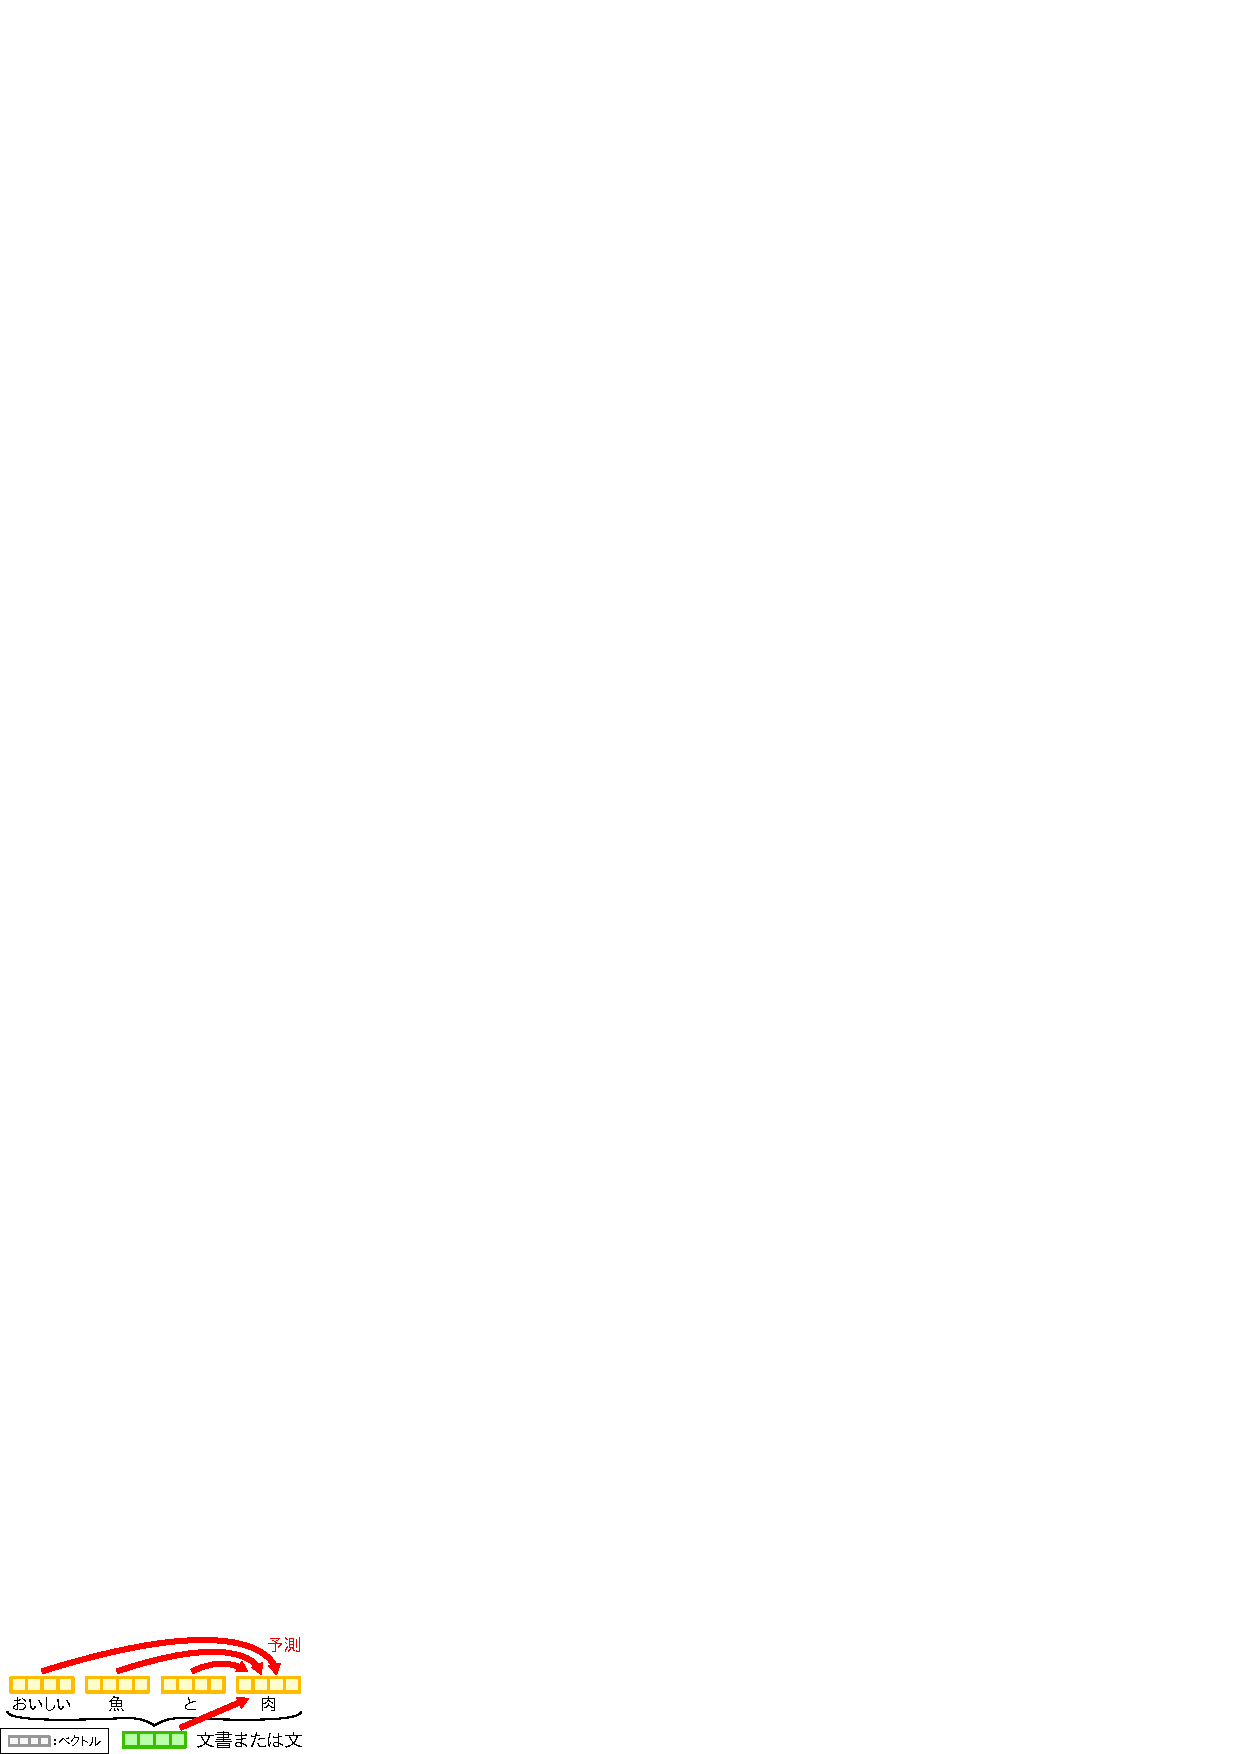
\includegraphics[0.5]{fig/paragraph_vector_v2.pdf}
  \caption{パラグラフベクトルの学習の概略}
  \label{fig:ParagraphVector}
\end{figure}

以下に具体的なアルゴリズムを示す。
ここでは文書の意味表現を学習する場合について考える。
学習の概略を図\ref{fig:ParagraphVector}に示す。
まず、意味表現を学習する対象となる文書に含まれる単語を
初めから一つずつ読んでいく。
その際、現在の単語及びその周辺の単語、現在の文書について、
式\ref{eq:ParagraphVector}に示す目的関数$L$を最大化するように
各パラメータの学習を行う。
\begin{gather}
  L = \frac{1}{T} \sum^{T}_{t = k} \log p(w_t | w_{t-k}, ..., w_{t-1}),
    \label{eq:ParagraphVector} \\
  p(w_t | w_{t-k}, ..., w_{t-1}) = \frac{e^{y_{w_t}}}{\sum_i e^{y_i}},
    \nonumber \\
  y = b + Uh(w_{t-k}, ..., w_{t-1}, d; W, D) \nonumber
\end{gather}
ここで、$d$は文書、$w_i$は単語、$W$は全ての単語の分散表現を表す行列、
$D$は全ての文書の分散表現を表す行列である。
$k$はウィンドウサイズ、$T$は現在の文書に含まれる単語数である。
ある単語の周辺を表す区間をウィンドウという。
$p$はsoftmax関数により正規化された、文脈から現在の単語が導かれることの
尤度である。
$p$を構成する$y$は現在の単語とウィンドウ内の単語及び現在の文書から導出される。
$h(w_{t-k}, ..., w_{t-1}, d; W, D)$は引数となるベクトルを平均したベクトル
または結合したベクトルを返す関数である。

PV-DMによって得られたパラグラフベクトルはレーティング予測において
BOW等に比べ高い正答率を示すことが示されている。
しかし、文書全体にパラグラフベクトルを用いる場合、文同士の位置関係が
予測時に考慮できない。


\subsection{ニューラルネットワークを用いた評判分析}

ニューラルネットワークを用いた評判分析の手法が、Nalら\cite{nal14}、
Rieら\cite{rie14}、Duyuら\cite{duyu15}等によって提案されている。
これらの方法に共通するのは、単語の意味表現から畳み込みニューラルネットワークと
全結合ニューラルネットワークを用いて分類を行うことである。
まず、単語の意味表現から畳み込みニューラルネットワークを
用いて単語同士の関係を捉えた特徴量を抽出する。
その後、そこから得られた文書全体の特徴量を
全結合ニューラルネットワークの入力とし多値または二値分類を行う。
また、Duyuら\cite{duyu15}とNalら\cite{nal14}の手法は
ニューラルネットワークのモデルの中にパラメータとして
単語の意味表現を取り込んでいる。
これにより、特定の分類問題に対してそれらを最適化することができる。

これらの手法は1つのカテゴリにおける多値または二値分類を対象としている。
よって、多カテゴリのレーティング予測において、これらの手法をカテゴリ毎に
適用しただけではカテゴリ間の関係を考慮することができない。

\section{提案手法} \label{sec:ProposedMethod}

提案手法では、パラグラフベクトルによってレビュー内の各文及び文章の意味表現を
生成し、それらをニューラルネットワークの入力として分類を行う。
以下にその基礎となるアイデアと具体的なアルゴリズムを示す。


\subsection{文書・文間及びカテゴリ間の関係の考慮}

先行研究\cite{fujitani15}の実験結果から、
レビュー内の文毎の素性を元にレビューの分類を行うことが
正答率の向上に有効であると考えられる。
また、カテゴリ間の繋がりの変化が正答率に影響していることから、
これをパラメータとして機械学習のモデルに組み込めば
正答率を向上させることができると考えられる。
さらに、レビュー内の文毎に意味表現を生成し分類器の入力とすることで、
その順序を考慮した学習を行う。

以下に、文の位置関係が重要となる例を示す。
2つ目の例は、1つ目の例の2つ目の文と3つ目の文を入れ替えたものである。
\begin{addmargin}{8ex}
  \vspace{1em}
  \setstretch{1}
  食事が美味しかった。
  とても良かった。
  部屋から眺めが素晴らしかった。
\end{addmargin}
\begin{addmargin}{8ex}
  \vspace{1em}
  \setstretch{1}
  食事が美味しかった。
  部屋から眺めが素晴らしかった。
  \textbf{とても良かった。}
\end{addmargin}
1つ目の例では、「とても良かった。」という文が直前の食事に関する文の
意味を補完しているのに対し、
2つ目の例では、部屋に関する文の意味を補完している。
このように、文の位置関係によってどの文がどの文と強く関連しているかが変化する。
それによって、予測すべきレビュー全体のレーティングも変化する。
よって、文の位置関係を考慮することは重要である。

次に、カテゴリ間の関係が重要となる例を
図\ref{fig:RelationsAmongRatingCategories}に示す。
図\ref{fig:RelationsAmongRatingCategories}のように
「総合」カテゴリのレーティングは一般に他のカテゴリのレーティングに応じて
高くなる。
このような関係は「立地」と「部屋」、「食事」と「サービス」等の
他のカテゴリ間にも存在する。
よって、このことからも、カテゴリ間の関係をレーティング予測において
考慮することで、正答率を向上させられると考えられる。

\begin{figure}
  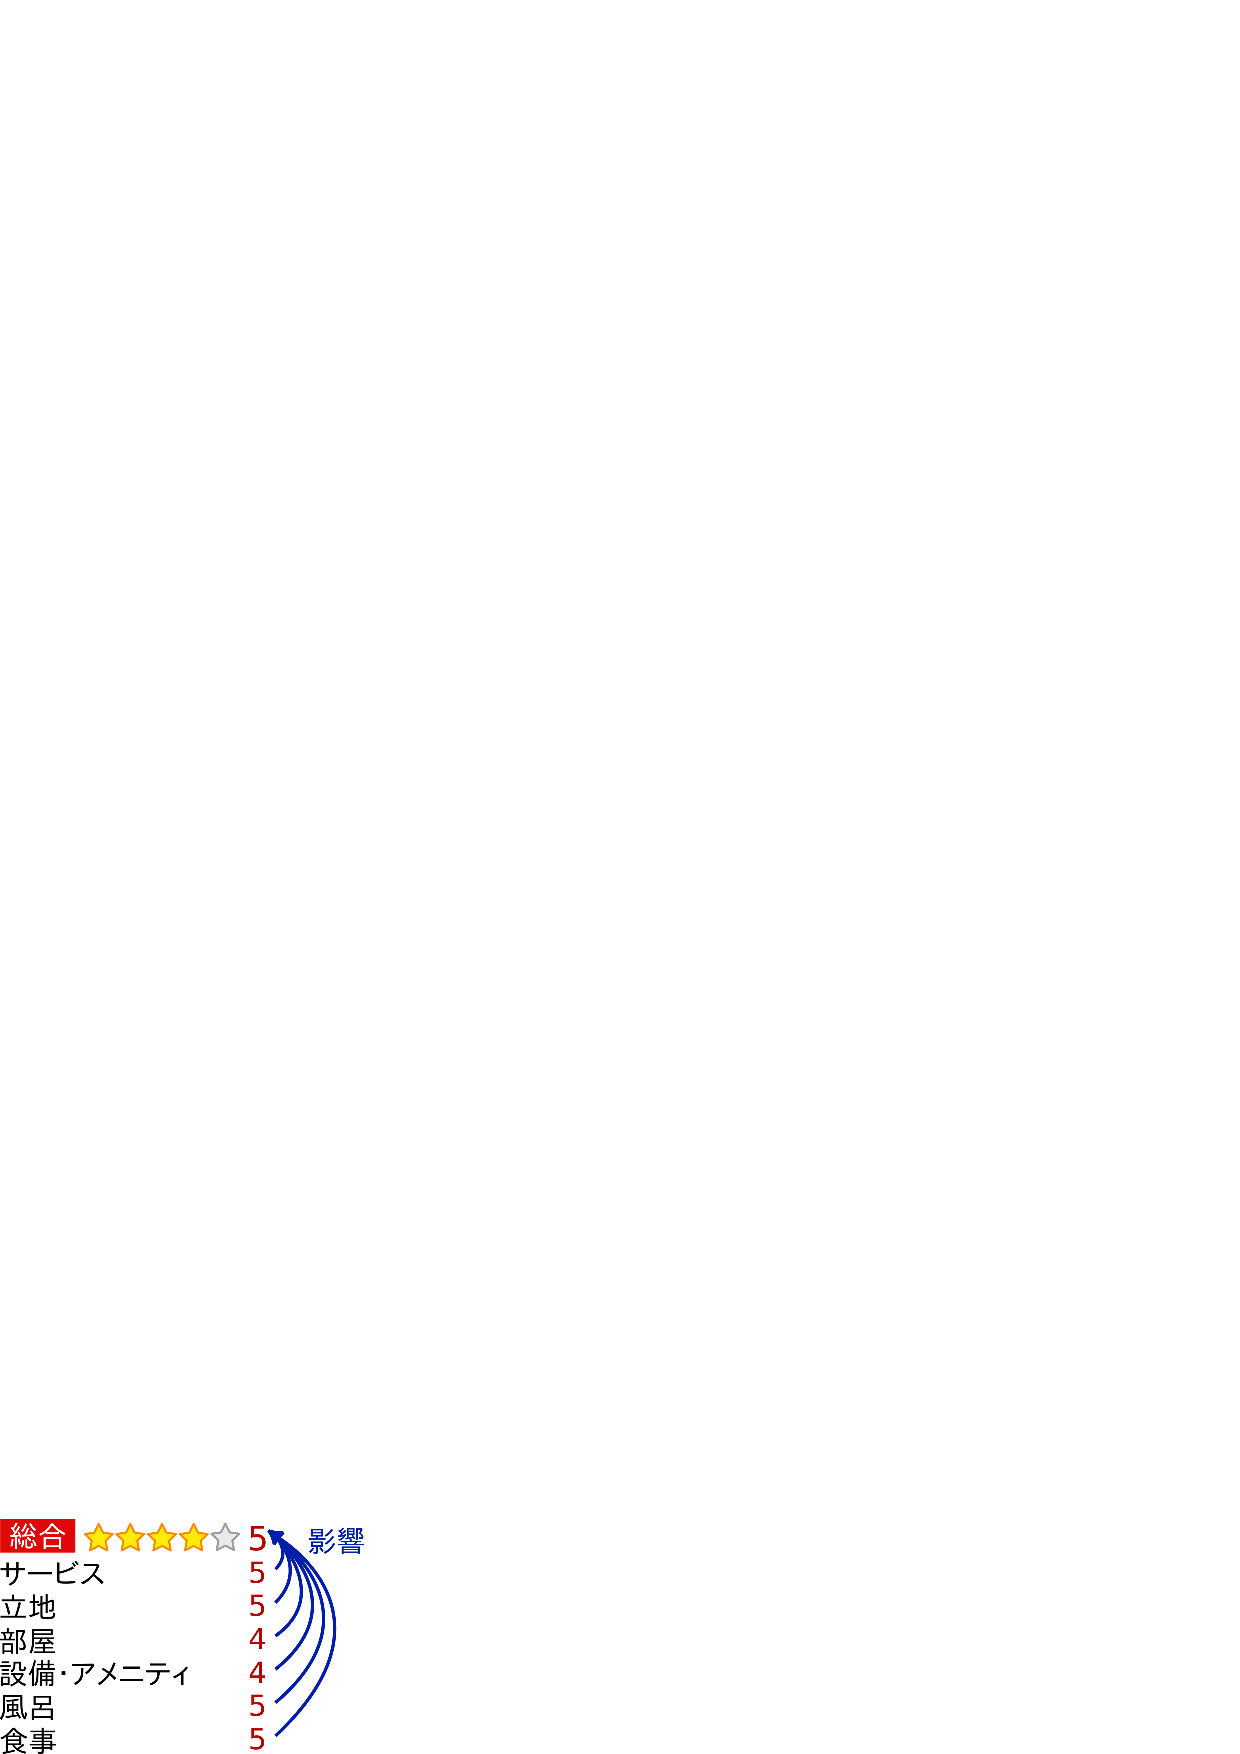
\includegraphics[0.3]{fig/relations_among_rating_categories.pdf}
  \caption{カテゴリ間の関係の例}
  \label{fig:RelationsAmongRatingCategories}
\end{figure}

しかし、個々のレビューに対して全ての文ベクトルを
ニューラルネットワークによる分類器の入力とすることは問題がある。
なぜならば、文の数はレビュー毎に異なっており、
複数レビュー内の複数の文ベクトルを単純な行列として表せないためである。
これは、分類器のミニバッチ方式の訓練を難しくし、
プログラムの実行時間を増加させる。
この問題に対処するため、本手法では各レビュー内の文ベクトルに対して
重み付け平均を行う。
これにより、全てのレビューで文ベクトルの数が統一され、
複数レビュー内の複数の文ベクトルをまとめて3次元行列として表すことができる。
つまり、ミニバッチ方式の訓練における計算が容易となる。

分類器はニューラルネットワークを用いて構成することによって、
文書・文間の関係とカテゴリ間の関係を同時に捉えた分類を行う。
従来手法\cite{nal14}や\cite{rie14}、\cite{duyu15}では、
単語ベクトルに対して畳込みニューラルネットワークが用いられている。
しかし、提案手法においては、畳み込みニューラルネットワークより
全結合ニューラルネットワークを用いた方が正答率が高かったため、
分類器には後者のみを用いた。


\subsection{アルゴリズム}

提案手法の処理の流れを説明する。
図\ref{fig:MyAlgorithm}にアルゴリズム全体の概略を示す。

\begin{figure}
  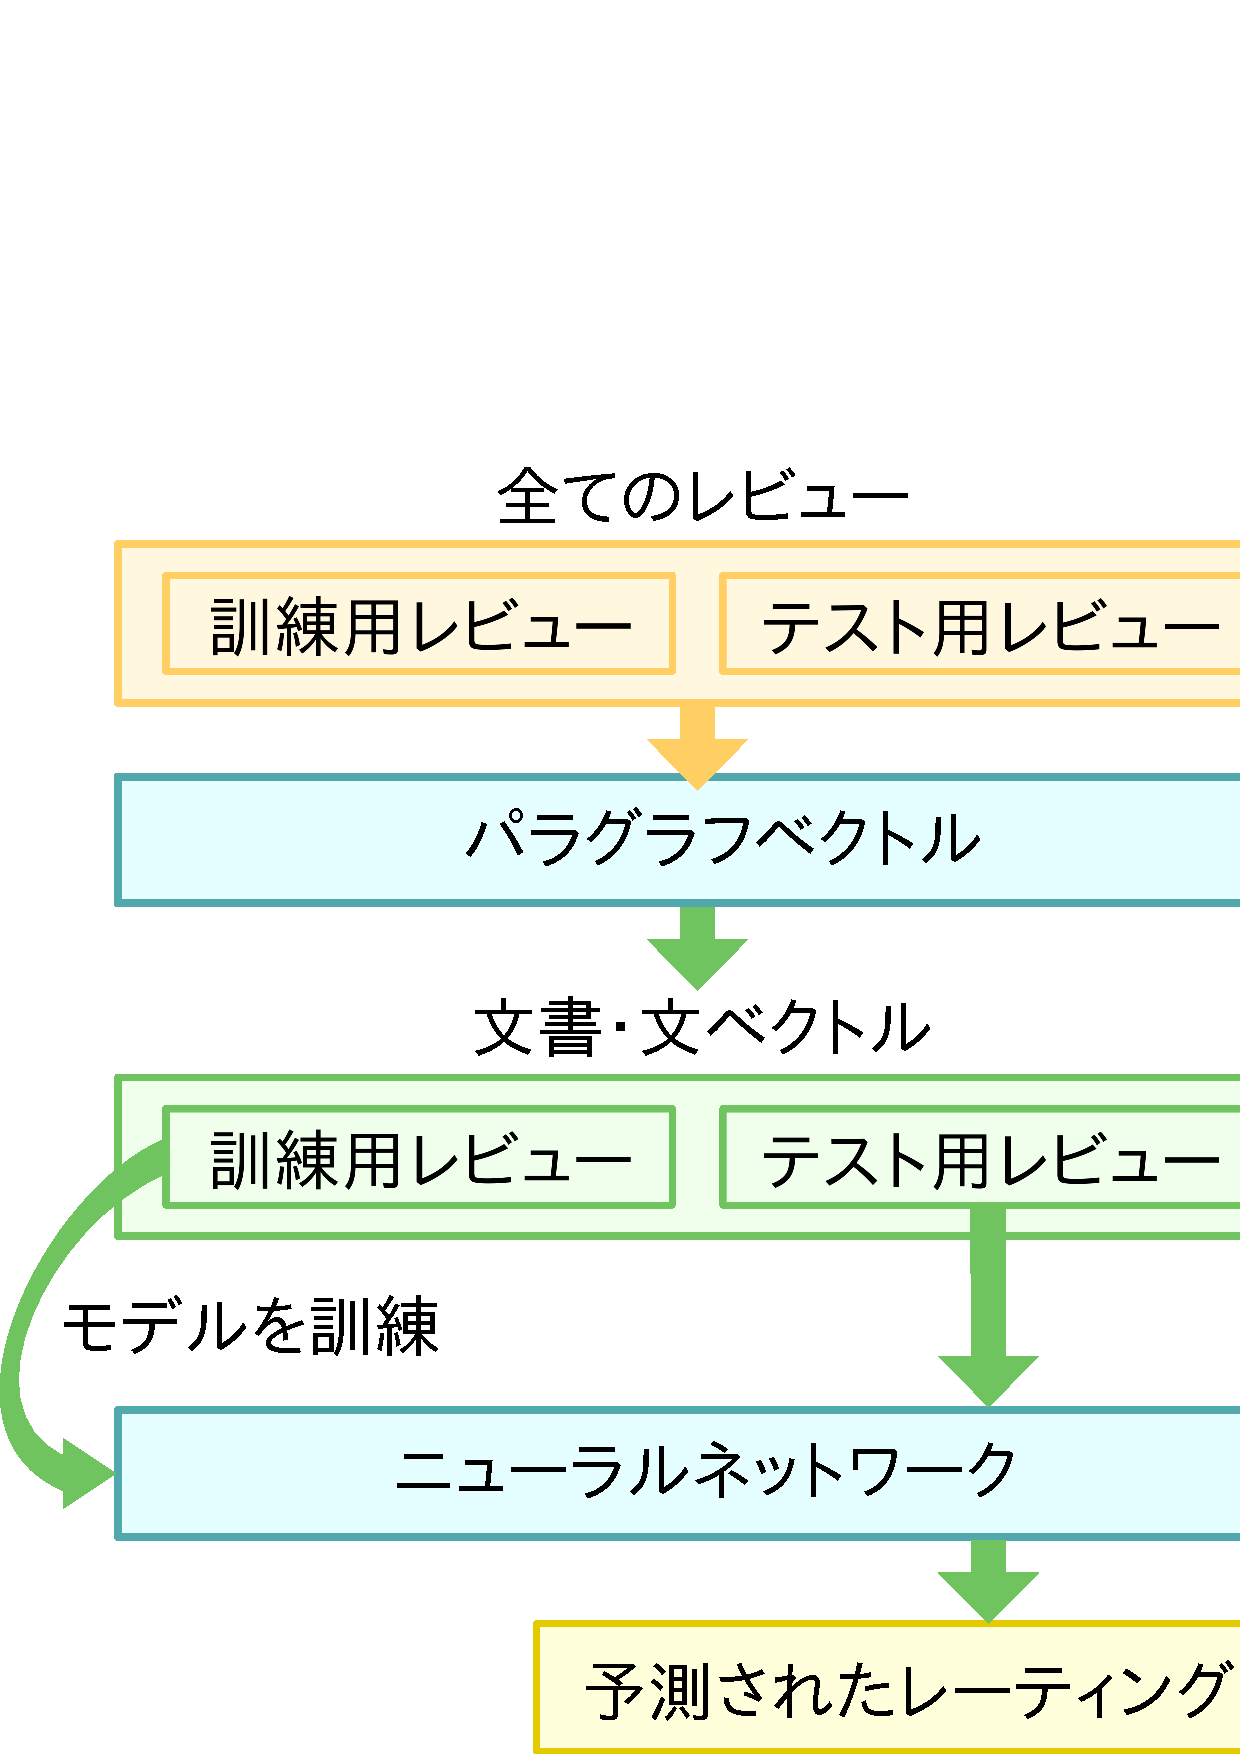
\includegraphics[0.5]{fig/algorithm.pdf}
  \caption{提案手法におけるアルゴリズムの概略}
  \label{fig:MyAlgorithm}
\end{figure}

%提案手法では、PV-DMによってレビュー内の文書全体及び各文の意味表現を
%生成し、それらをニューラルネットワークの入力として分類を行う。
%文毎の意味表現を用いることで文同士の位置関係を考慮し、
%ニューラルネットワークによる分類器を用いることで
%文間及びカテゴリ間の深い関係性を捉えることを目指す。
%提案手法の入力はレビューである文書と正解レーティングの組の集合、
%出力は各文書について予測されたカテゴリ毎のクラスである。
%以下に提案手法の処理の流れを示す。

初めに、PV-DMを用いて、
各レビューの文書全体のベクトルとそれに含まれる各文のベクトルを生成する。
以降、これらをそれぞれ文書ベクトル、文ベクトルと呼ぶ。
文書ベクトルと文ベクトルについては別々に学習し生成する。
%式\ref{eq:PVObjective}に示す目的関数$L_d$を最大化するように学習を行う。
%\begin{multline}
%  L_d = \sum^{T}_{t = n + 1} \{ \log \sigma(s(w_t, w_{t-n}, ..., w_{t-1}, d)) \\
%        + \sum^{k}_{w_{t}' \sim P_n}
%        \log(1 - \sigma(s(w_{t}', w_{t-n}, ..., w_{t-1}, d))) \},
%    \label{eq:PVObjective} \\
%\end{multline}
%\begin{gather}
%  s(w_t, w_{t - n}, ..., w_{t - 1}, d)
%    = W_{map}(w_t)
%      \cdot \begin{bmatrix} W(w_{t - n}) \\ \vdots
%      \\ W(w_{t - 1}) \\ D(d) \end{bmatrix} \nonumber
%\end{gather}
%ここで、$T$は現在の文章内の単語数、$t$は現在の単語位置、$d$は現在の文章、
%$w_i$は位置$i$にある単語、$n$はウィンドウサイズである。
%$W(w_i)$は単語$w_i$に相当する単語ベクトルを単語行列$W$から抜き出す関数を表す。
%$D(d)$は文章$d$に相当する文章ベクトルを文章行列$D$から抜き出す関数を表す。
%関数$s(w_t, w_0, ..., w_n, d)$はある単語とそれが出現する文脈との類似度を
%計算する。
%行列$W_{map}$は内積によって文脈と単語との類似度を計算するための単語毎
%のベクトルを保持する。
%文章行列内の各文章ベクトルはレビュー全体を表す文書ベクトル、または、
%各レビュー内の文ベクトルを表す。
%$\sigma$はシグモイド関数である。
%また、式\ref{eq:PVObjective}の中括弧内の右項はネガティブサンプリングを
%表す。
%ネガティブサンプリングとは、文脈外の単語をデータセットにおける出現確率で
%サンプリングし、それらと文脈の意味が遠ざかるように学習する手法である。
%$w_{t}' \sim P_n$は文脈外の単語$w_{t}'$を単語の出現頻度$P_n$によって
%サンプリングすることを示す。
%ただし、出現頻度は極端に頻出する単語の影響を抑えるため
%各単語に対して3/4乗している。
%現在の単語と同じ単語や同一回の学習で一度サンプリングされた単語は
%サンプリングしない。
式\ref{eq:ParagraphVector}の目的関数における$h$には
引数のベクトルを結合する関数を用いる。
また、学習の高速化のため、Quocら\cite{quoc14}によって
用いられている階層的softmax関数の代替として、ネガティブサンプリングを行う。
ネガティブサンプリングとは、文脈外の単語をデータセットにおける出現確率で
サンプリングし、それらと文脈の意味が遠ざかるように学習する手法である。
ただし、出現頻度は極端に頻出する単語の影響を抑えるため
各単語に対して3/4乗している。
現在の単語と同じ単語や同一回の学習で一度サンプリングされた単語は
サンプリングしない。

次に、各レビュー内の全ての文ベクトルに対して重み付け平均を行い、
圧縮された文ベクトルを生成する。
この過程により、各レビューで疎らだった文の数を統一する。
式\ref{eq:WeightedAverageSV}に重み付け平均によって圧縮した
文ベクトル$t_{i_{part}}$を示す。
各文ベクトルは圧縮後の各文ベクトルと位置が近いほど重みが大きくなるように
重み付け平均する。
\begin{gather}
  \mathbf{t}_{i_{part}} = \sum_{i_{sent}}
                          \frac{w(x_{i_{part}}(i_{sent}))}
                               {|\sum_{i_{sent}'}
                                w(x_{i_{part}}(i_{sent}'))|}
                          \mathbf{s}_{i_{sent}},
  \label{eq:WeightedAverageSV} \\
  x_{i_{part}}(i_{sent}) = \frac{i_{sent}}{\#sent - 1}
                           - \frac{i_{part}}{\#part - 1}, \nonumber \\
  w(x) = \begin{cases}
    \frac{1}{2} (\cos(\pi|x|) + 1) & \text{if $|x| \leq 1$} \\
    0 & \text{otherwise}
  \end{cases} \nonumber
\end{gather}
ここで、$\mathbf{s}_{i_{sent}}$はレビュー内の文ベクトル、
$\mathbf{t}_{i_{part}}$は重み付け平均された文ベクトルである。
$i_{sent}$はレビュー内の文ベクトルのインデックス、
$i_{part}$は重み付け平均された文ベクトルのインデックスである。
$\#sent$はレビュー内の文ベクトルの数、
$\#part$は重み付け平均された文ベクトルの数である。
\footnote{
  重み付けの関数には$\cos$関数の他に、
  $x$に対して線形に重みを減少させるような関数や、
  単純に文を区画毎に平均するような関数も考えられる。
  区画毎に平均する関数は他の2つより正答率が低く、線形な関数と
  $\cos$関数はほぼ同じ正答率を示したため、$\cos$関数を採用した。
}

最後に、分類器によってレーティング予測を行う。
分類器は全結合ニューラルネットワークによって構成される。
図\ref{fig:MyModel}に各層の結合の様子を示す。
\begin{figure}
  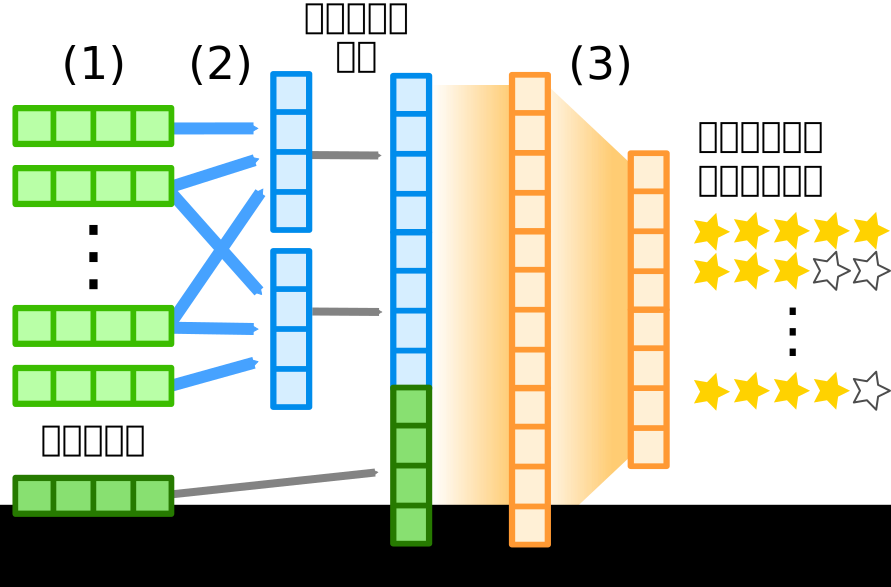
\includegraphics[0.6]{fig/model_with_formal_process_numbers.pdf}
  \caption{全結合ニューラルネットワークによる分類器}
  \label{fig:MyModel}
\end{figure}
入力層はレビュー毎の文書ベクトルと圧縮された文ベクトルの結合ベクトルである。
ニューラルネットワークの活性化関数には、シグモイド関数を用いる。
また、出力層はカテゴリの数とレーティングの場合の数の積だけのニューロンを持ち、
各ニューロンの出力はあるカテゴリ内であるレーティング値が選ばれることの
正規化されていない対数確率を表す。
ニューラルネットワークは式\ref{eq:NNObjective}に示す目的関数$E$を
最小化するように学習を行う。
\begin{gather}
  E = - \sum^{N}_{n = 1} \sum^{C}_{c = 1} \sum^{K}_{k = 1}
        d_{nck} \log{y_{ck}(x_n; w)},
  \label{eq:NNObjective} \\
  y_{ck}(x_n; w) = \frac{e^{u_{ck}(x_n; w)}}
                        {\sum^{K}_{j = 0} e^{u_{cj}(x_n; w)}} \nonumber
\end{gather}
各ニューロンの出力はカテゴリ毎に交差エントロピー誤差関数によって
損失に変換される。
ここで、$u_{ck}$は出力層のニューロンの出力値、$y_{ck}$はカテゴリ$c$において
クラス$k$が選ばれる確率、$w$はニューラルネットワークのパラメータである。
$d_{nck}$は$n$番目の文書がカテゴリ$c$でクラス$k$ならば1、
それ以外で0となる値である。
$N$はミニバッチサイズ、$C$はカテゴリの総数、$K$はクラスの総数である。
ところで、ニューラルネットワークによる多値分類では一般に、
出力層のニューロンの値である対数確率全てをsoftmax関数で
正規化する。
しかし、複数カテゴリの多値分類問題において、
同様に出力層のニューロンの値を正規化してしまうと
softmax関数の値が確率としての意味を成さない。
よって、式\ref{eq:NNObjective}では、
カテゴリ毎にsoftmax関数でニューロンの出力値が示す対数確率を正規化する。
そして、それらを各カテゴリの目的関数とし、足し合わせることで
あるレビューに対する目的関数を構成する。
これを全てのレビューに対して足し合わせ、
ニューラルネットワークの目的関数とする。
さらに、ニューラルネットワークの学習時にはドロップアウト及び重み減衰を行う。
ただし、重み減衰において全結合層の重みの内、バイアスは減衰していない。
パラメータ最適化の手法にはAdam\cite{diederik15}を用いる。

\section{実験}

\subsection{実験設定}

実験は、各手法の正答率を測定するものと、提案手法における予測レーティングと
正解レーティングの平均二乗誤差(RMSE)を測定するものの2つを行った。
RMSEの計算において、正解または予測レーティングが0点であるものは評価から省いた。
比較手法として、
提案手法における分類器の入力をそれぞれ
(1) DV (Document Vector)、
(2) ASV (Averaged Sentence Vector)、
(3) Weighted ASV
に変えた手法を用いた。
DVとはレビュー全体の文書ベクトルであり、
Quocら\cite{quoc14}の手法に相当する。
ASVとはレビュー内で平均した文ベクトルであり、
Weighted ASVとはレビュー内で重み付け平均によって圧縮された文ベクトルである。
データセットとしては、先行研究\cite{fujitani15}と同様に、
ホテル予約サイト楽天トラベルにおけるレビュー337,266件からレビューの番号順に
訓練データ300,000件、開発データ10,000件、評価データ10,000件を用いた。
有意差検定にはマクネマー検定を用い、
p値が0.05より小さいとき有意とした。

%比較手法として、
%及び、提案手法における分類器の入力を変えた2つの手法、
%(1) Quocら\cite{quoc14}によるDV、
%(2) ASV (Averaged Sentence Vector)
%と
%(3) Weighted ASVを用いた。
%これらの手法と提案手法に用いる分類器の入力を
%表\ref{tab:MethodFeatures}に列挙する。

%\begin{table}
%  \caption{各手法に用いられる特徴量}
%  \centering
%  \begin{tabularx}{\linewidth}{l | X} \label{tab:MethodFeatures}
%    手法 & 特徴量 \\
%    \hline
%    DV & レビュー全体の文書ベクトル \\
%    \hline
%    ASV & レビュー内で平均した文ベクトル \\
%    \hline
%    Weighted ASV & レビュー内で重み付け平均によって圧縮された文ベクトル \\
%    \hline
%    提案手法 & レビュー全体の文書ベクトル、\\
%             & レビュー内で重み付け平均によって圧縮された文ベクトル \\
%  \end{tabularx}
%\end{table}

%ASVとWeighted ASVの比較によって、
%文の位置関係が分類に対して重要であるかが示される。
%基準手法と提案手法、また、Weighted ASVと提案手法の基準手法の比較によって、
%文書ベクトルと文ベクトルを同時に特徴量として用いることが
%有効であるかが示される。

表\ref{tab:ParametersOfMethods}に各手法におけるニューラルネットワークの
パラメータ設定を示す。
全ての手法において、中間層の数は1、入力層及び中間層におけるドロップアウト率は
それぞれ0.2と0.5で共通である。
Adam\cite{diederik15}のハイパーパラメータは\cite{diederik15}と同様の値を
用いた。
Weighted ASVと提案手法において圧縮された文ベクトルの数は
それぞれ3つと2つとした。
全ての実験において文書及び文ベクトルについては、
学習回数は1,024回、学習する単語の範囲は前3単語、単語の最少出現回数は5回、
ネガティブサンプリングの回数は5回、ベクトルの次元数は600次元に
設定し学習したものを用いた。

\begin{table}
  \caption{各手法のパラメータ設定}
  \centering
  \begin{tabular}{l | r r} \label{tab:ParametersOfMethods}
    手法 & 学習回数 & 中間層でのユニット数 \\
    \hline
    DV & 20 & 512 \\
    ASV & 55 & 256 \\
    Weighted ASV & 24 & 256 \\
    提案手法 & 30 & 512 \\
  \end{tabular}
\end{table}

レビューに対する前処理について以下に示す。
まず、レビューの文書に対して、文字の正規化処理を行った。
記号「!”#$%&’()*+,−./:;<>?@[¥]^_`{|}
\unicode{301C}」は全てNFKC形式で正規化した。
記号「\unicode{02D7}\unicode{058A}\unicode{2011}\unicode{2012}\unicode{2013}
\unicode{2043}\unicode{207B}\unicode{208B}\unicode{2212}」
は全て記号「-」で置き換えた。
記号「\unicode{FE63}-ー—―─━ー」は全て記号「ー」で置き換えた。
チルダ記号「\unicode{007E}\unicode{223C}\unicode{223E}\unicode{301C}
\unicode{3030}\unicode{FF5E}」は全て削除した。
次に、文の解析は正規表現を用いて行った。
「。」、「.」、「!」、「?」を文の終端文字とし、
解析した最後の文の次の文字から
文の終端文字または文書の終端までを一つの文として解析した。
最後に、形態素解析には形態素解析器MeCabを用いた、
辞書にはIPA辞書を用いた。
単語の情報は表層のみを利用し、表層が無いものは取り除いた。


\subsection{結果}

まず、提案手法と3つの比較手法、従来手法\cite{fujitani15}を
正答率で比較したものを表\ref{tab:Accuracies}に示す。
また、表\ref{tab:AccuraciesPerCategory}に提案手法と
従来手法\cite{fujitani15}におけるカテゴリ別の正答率を示す。
表\ref{tab:Accuracies}において、
提案手法が従来手法\cite{fujitani15}の正答率を0.0198有意に上回っている。
また、提案手法がDVの正答率を0.0050有意に上回っている。
Weighted ASVがASVを0.029有意に上回っている。

\begin{table}
  \caption{各手法における正答率}
  \centering
  \begin{tabular}{l | r} \label{tab:Accuracies}
    手法 & 正答率 \\
    \hline
    従来手法\cite{fujitani15} & 0.4832 \\
    DV & 0.4980 \\
    ASV & 0.4838 \\
    Weighted ASV & 0.4867 \\
    提案手法 & \textbf{0.5030} \\
  \end{tabular}
\end{table}

\begin{table}
  \caption{提案手法と従来手法\cite{fujitani15}におけるカテゴリ別の正答率}
  \centering
  \begin{tabular}{l | r r r r r r r} \label{tab:AccuraciesPerCategory}
    手法 & 立地 & 部屋 & 食事 & 風呂 & サービス & 設備 & 総合 \\
    \hline
    提案手法 & 0.5140 & 0.4984 & 0.5353 & 0.4347 & 0.5116 & 0.4479 & 0.5794 \\
    従来手法\cite{fujitani15}
        & 0.4961 & 0.4706 & 0.5140 & 0.3973 & 0.4783 & 0.4265 & 0.5660 \\
  \end{tabular}
\end{table}

次に、表\ref{tab:RMSEs}にレーティングのRMSEを測定した結果を示す。
提案手法は従来手法\cite{fujitani15}が弱点としていた
食事と風呂のカテゴリにおいてそれぞれ0.60及び0.24だけ低い誤差を示した。
また、その他全てのカテゴリにおいても提案手法は従来手法より低い誤差を示した。

\begin{table}
  \caption{提案手法と従来手法\cite{fujitani15}におけるレーティングのRMSE}
  \centering
  \begin{tabular}{l | r r} \label{tab:RMSEs}
    手法 & 提案手法 & 従来手法\cite{fujitani15} \\
    \hline
    立地      & 0.88 & 0.97 \\
    部屋      & 0.88 & 0.97 \\
    食事      & 0.93 & 1.53 \\
    風呂      & 1.03 & 1.27 \\
    サービス  & 0.86 & 0.94 \\
    設備      & 0.90 & 0.95 \\
    総合      & 0.73 & 0.81 \\
  \end{tabular}
\end{table}

最後に、正答率を測定する実験における提案手法の精度と再現率、F値を
それぞれ表\ref{tab:ProposedMethodPrecision}と
表\ref{tab:ProposedMethodRecall}、表\ref{tab:ProposedMethodFValue}に示す。
表においてnanは0による除算が発生し計算できなかったことを示す。

\begin{table}
  \caption{提案手法の精度}
  \centering
  \begin{tabular}{l | r r r r r r r | r} \label{tab:ProposedMethodPrecision}
    レーティング & 立地 & 部屋 & 食事 & 風呂 & サービス & 設備 & 総合
      & 全カテゴリ \\
    \hline
    \csvreader[no head,late after line=\\]
      {csv/class_precision.csv}
      {1=\rating,2=\location,3=\room,4=\mean,5=\bath,6=\service,7=\facilities,
       8=\overall,9=\allcategories}
      {\rating & \location & \room & \mean & \bath & \service & \facilities
       & \overall & \allcategories}
  \end{tabular}
\end{table}

\begin{table}
  \caption{提案手法の再現率}
  \centering
  \begin{tabular}{l | r r r r r r r | r} \label{tab:ProposedMethodRecall}
    レーティング & 立地 & 部屋 & 食事 & 風呂 & サービス & 設備 & 総合
      & 全カテゴリ \\
    \hline
    \csvreader[no head,late after line=\\]
      {csv/class_recall.csv}
      {1=\rating,2=\location,3=\room,4=\mean,5=\bath,6=\service,7=\facilities,
       8=\overall,9=\allcategories}
      {\rating & \location & \room & \mean & \bath & \service & \facilities
       & \overall & \allcategories}
  \end{tabular}
\end{table}

\begin{table}
  \caption{提案手法のF値}
  \centering
  \begin{tabular}{l | r r r r r r r | r} \label{tab:ProposedMethodFValue}
    レーティング & 立地 & 部屋 & 食事 & 風呂 & サービス & 設備 & 総合
      & 全カテゴリ \\
    \hline
    \csvreader[no head,late after line=\\]
      {csv/class_f_value.csv}
      {1=\rating,2=\location,3=\room,4=\mean,5=\bath,6=\service,7=\facilities,
       8=\overall,9=\allcategories}
      {\rating & \location & \room & \mean & \bath & \service & \facilities
       & \overall & \allcategories}
  \end{tabular}
\end{table}

\section{結論}

本研究では、多カテゴリにおける評判分類問題について、
レビュー全体の文書ベクトルに加え重み付け平均された文ベクトルを用いた手法を
提案した。

実験では、提案手法が従来手法\cite{fujitani15}より高い正答率を示した。
また、比較手法の結果より、
レビュー内の文の並びが評判分類に重要であること、及び、
文書ベクトルと文ベクトルがレビューのいくらか異なる特徴を捉えていることが
分かった。

今後の課題は言語要素間のより多様で複雑な関係を考慮することである。
このためには、各レビューの意味表現を生成するモデルと
分類を行うモデルを1つに統合する必要がある。
なぜならば、モデルが分かれていることによって
単語や文字などのより小さな言語要素同士の関係を分類時に考慮できないためである。
モデルの統合によって、学習手法の柔軟性を高めると共に
さらなる正答率の向上を目指す。


%今後の課題は、提案手法の中で2つに分かれているモデルの統合である。
%
%提案手法は、分類すべき文書とそれが含む文の分散表現を生成する段階、及び、
%それらを用いて分類を行う段階の2つの段階に分かれている。
%このことは、問題を2つに分けることで個々の問題を単純にしているが、
%同時に文書の分類を一つずつ行うことを難しくしている。
%また、文書や文の分散表現を事前に生成するための
%PV-DMのパラメータは、実際には最大の正答率を達成するため
%分類器のパラメータとして最適化されることが望ましい。
%
%今後は、これらの問題を解決するために、文書や文の分散表現を生成する過程を
%ニューラルネットワークによる分類器に統合する。
%これによって、学習方法の柔軟性を高めると共にさらなる正答率の向上を目指す。



\section*{謝辞}
本研究において、楽天株式会社よりホテル予約サイト楽天トラベルにおける
レビューデータを使用させていただきました。
この場を借りて深く感謝致します。



\bibliographystyle{jplain}
\begin{thebibliography}{9}
\bibitem{fujitani15}
  藤谷宣典ら,
  隠れ状態を用いたホテルレビューのレーティング予測.
  言語処理学会第21回年次大会, 2015.
\bibitem{quoc14}
  Quoc Le, and Tomas Mikolov,
  Distributed Representations of Sentences and Documents.
  ICML 2014, 2014.
\bibitem{nal14}
  Nal Kalchbrenner, Edward Grefenstette, and Phil Blunsom,
  A Convolutional Neural Network for Modelling Sentences.
  ACL 2014, 2014.
\bibitem{rie14}
  Rie Johnson, and Tong Zhang,
  Effective Use of Word Order for Text Categorization
  with Convolutional Neural Networks.
  NAACL 2015, 2015.
\bibitem{duyu15}
  Duyu Tang, Bing Qin, and Ting Liu,
  Learning Semantic Representation of Users and Products
  for Document Level Sentiment Classification.
  ACL 2015, 2015.
\bibitem{yoshua03}
  Yoshua Bengio et al,
  A Neural Probabilistic Language Model.
  The Journal of Machine Learning Research 3, 2003.
\bibitem{mihai12}
  Mihai Surdeanu et al,
  Multi-instance Multi-label Learning for Relation Extraction.
  CoNLL 2012, 2012.
\end{thebibliography}

\end{document}
